\documentclass{ximera}

\usepackage{epsfig}

\graphicspath{
  {./}
  {figures/}
}

\usepackage{epstopdf}
%\usepackage{ulem}
\usepackage[normalem]{ulem}

\epstopdfsetup{outdir=./}

\usepackage{morewrites}
\makeatletter
\newcommand\subfile[1]{%
\renewcommand{\input}[1]{}%
\begingroup\skip@preamble\otherinput{#1}\endgroup\par\vspace{\topsep}
\let\input\otherinput}
\makeatother

\newcommand{\EXER}{}
\newcommand{\includeexercises}{\EXER\directlua{dofile(kpse.find_file("exercises","lua"))}}

\newenvironment{computerExercise}{\begin{exercise}}{\end{exercise}}

%\newcounter{ccounter}
%\setcounter{ccounter}{1}
%\newcommand{\Chapter}[1]{\setcounter{chapter}{\arabic{ccounter}}\chapter{#1}\addtocounter{ccounter}{1}}

%\newcommand{\section}[1]{\section{#1}\setcounter{thm}{0}\setcounter{equation}{0}}

%\renewcommand{\theequation}{\arabic{chapter}.\arabic{section}.\arabic{equation}}
%\renewcommand{\thefigure}{\arabic{chapter}.\arabic{figure}}
%\renewcommand{\thetable}{\arabic{chapter}.\arabic{table}}

%\newcommand{\Sec}[2]{\section{#1}\markright{\arabic{ccounter}.\arabic{section}.#2}\setcounter{equation}{0}\setcounter{thm}{0}\setcounter{figure}{0}}
  
\newcommand{\Sec}[2]{\section{#1}}

\setcounter{secnumdepth}{2}
%\setcounter{secnumdepth}{1} 

%\newcounter{THM}
%\renewcommand{\theTHM}{\arabic{chapter}.\arabic{section}}

\newcommand{\trademark}{{R\!\!\!\!\!\bigcirc}}
%\newtheorem{exercise}{}

\newcommand{\dfield}{{\sf SlopeField}}

\newcommand{\pplane}{{\sf PhasePlane}}

\newcommand{\PPLANE}{{\sf PHASEPLANE}}

% BADBAD: \newcommand{\Bbb}{\bf}. % Package amsfonts Warning: Obsolete command \Bbb; \mathbb should be used instead.

\newcommand{\R}{\mbox{$\mathbb{R}$}}
\let\C\relax
\newcommand{\C}{\mbox{$\mathbb{C}$}}
\newcommand{\Z}{\mbox{$\mathbb{Z}$}}
\newcommand{\N}{\mbox{$\mathbb{N}$}}
\newcommand{\D}{\mbox{{\bf D}}}

\newcommand{\WW}{\mathcal{W}}

\usepackage{amssymb}
%\newcommand{\qed}{\hfill\mbox{\raggedright$\square$} \vspace{1ex}}
%\newcommand{\proof}{\noindent {\bf Proof:} \hspace{0.1in}}

\newcommand{\setmin}{\;\mbox{--}\;}
\newcommand{\Matlab}{{M\small{AT\-LAB}} }
\newcommand{\Matlabp}{{M\small{AT\-LAB}}}
\newcommand{\computer}{\Matlab Instructions}
\renewcommand{\computer}{M\small{ATLAB} Instructions}
\newcommand{\half}{\mbox{$\frac{1}{2}$}}
\newcommand{\compose}{\raisebox{.15ex}{\mbox{{\scriptsize$\circ$}}}}
\newcommand{\AND}{\quad\mbox{and}\quad}
\newcommand{\vect}[2]{\left(\begin{array}{c} #1_1 \\ \vdots \\
 #1_{#2}\end{array}\right)}
\newcommand{\mattwo}[4]{\left(\begin{array}{rr} #1 & #2\\ #3
&#4\end{array}\right)}
\newcommand{\mattwoc}[4]{\left(\begin{array}{cc} #1 & #2\\ #3
&#4\end{array}\right)}
\newcommand{\vectwo}[2]{\left(\begin{array}{r} #1 \\ #2\end{array}\right)}
\newcommand{\vectwoc}[2]{\left(\begin{array}{c} #1 \\ #2\end{array}\right)}

\newcommand{\ignore}[1]{}


\newcommand{\inv}{^{-1}}
\newcommand{\CC}{{\cal C}}
\newcommand{\CCone}{\CC^1}
\newcommand{\Span}{{\rm span}}
\newcommand{\rank}{{\rm rank}}
\newcommand{\trace}{{\rm tr}}
\newcommand{\RE}{{\rm Re}}
\newcommand{\IM}{{\rm Im}}
\newcommand{\nulls}{{\rm null\;space}}

\newcommand{\dps}{\displaystyle}
\newcommand{\arraystart}{\renewcommand{\arraystretch}{1.8}}
\newcommand{\arrayfinish}{\renewcommand{\arraystretch}{1.2}}
\newcommand{\Start}[1]{\vspace{0.08in}\noindent {\bf Section~\ref{#1}}}
\newcommand{\exer}[1]{\noindent {\bf \ref{#1}}}
\newcommand{\ans}{\textbf{Answer:} }
\newcommand{\matthree}[9]{\left(\begin{array}{rrr} #1 & #2 & #3 \\ #4 & #5 & #6
\\ #7 & #8 & #9\end{array}\right)}
\newcommand{\cvectwo}[2]{\left(\begin{array}{c} #1 \\ #2\end{array}\right)}
\newcommand{\cmatthree}[9]{\left(\begin{array}{ccc} #1 & #2 & #3 \\ #4 & #5 &
#6 \\ #7 & #8 & #9\end{array}\right)}
\newcommand{\vecthree}[3]{\left(\begin{array}{r} #1 \\ #2 \\
#3\end{array}\right)}
\newcommand{\cvecthree}[3]{\left(\begin{array}{c} #1 \\ #2 \\
#3\end{array}\right)}
\newcommand{\cmattwo}[4]{\left(\begin{array}{cc} #1 & #2\\ #3
&#4\end{array}\right)}

\newcommand{\Matrix}[1]{\ensuremath{\left(\begin{array}{rrrrrrrrrrrrrrrrrr} #1 \end{array}\right)}}

\newcommand{\Matrixc}[1]{\ensuremath{\left(\begin{array}{cccccccccccc} #1 \end{array}\right)}}



\renewcommand{\labelenumi}{\theenumi}
\newenvironment{enumeratea}%
{\begingroup
 \renewcommand{\theenumi}{\alph{enumi}}
 \renewcommand{\labelenumi}{(\theenumi)}
 \begin{enumerate}}
 {\end{enumerate}
 \endgroup}

\newcounter{help}
\renewcommand{\thehelp}{\thesection.\arabic{equation}}

%\newenvironment{equation*}%
%{\renewcommand\endequation{\eqno (\theequation)* $$}%
%   \begin{equation}}%
%   {\end{equation}\renewcommand\endequation{\eqno \@eqnnum
%$$\global\@ignoretrue}}

%\input{psfig.tex}

\author{Martin Golubitsky and Michael Dellnitz}

%\newenvironment{matlabEquation}%
%{\renewcommand\endequation{\eqno (\theequation*) $$}%
%   \begin{equation}}%
%   {\end{equation}\renewcommand\endequation{\eqno \@eqnnum
% $$\global\@ignoretrue}}

\newcommand{\soln}{\textbf{Solution:} }
\newcommand{\exercap}[1]{\centerline{Figure~\ref{#1}}}
\newcommand{\exercaptwo}[1]{\centerline{Figure~\ref{#1}a\hspace{2.1in}
Figure~\ref{#1}b}}
\newcommand{\exercapthree}[1]{\centerline{Figure~\ref{#1}a\hspace{1.2in}
Figure~\ref{#1}b\hspace{1.2in}Figure~\ref{#1}c}}
\newcommand{\para}{\hspace{0.4in}}

\usepackage{ifluatex}
\ifluatex
\ifcsname displaysolutions\endcsname%
\else
\renewenvironment{solution}{\suppress}{\endsuppress}
\fi
\else
\renewenvironment{solution}{}{}
\fi

\ifcsname answer\endcsname
\renewcommand{\answer}{}
\fi

%\ifxake
%\newenvironment{matlabEquation}{\begin{equation}}{\end{equation}}
%\else
\newenvironment{matlabEquation}%
{\let\oldtheequation\theequation\renewcommand{\theequation}{\oldtheequation*}\begin{equation}}%
  {\end{equation}\let\theequation\oldtheequation}
%\fi

\makeatother

\newcommand{\RED}[1]{{\color{red}{#1}}} 


\title{RLC Circuits}

\begin{document}
\begin{abstract}
\end{abstract}
\maketitle

  \label{S:SOFE}
\index{RLC circuit}\index{electrical circuit}

RLC circuits provide an excellent example of a physical system that is well
modeled by a second order linear differential equation that is periodically 
forced by a discontinuous function.  Consider the electrical circuit shown in 
Figure~\ref{fig:rcl}.  The circuit consists of a resistor\index{resistor} with
resistance $R$, a coil\index{coil} with inductance $L$, a 
capacitor\index{capacitor} with 
capacitance $C$, and a voltage source\index{voltage source} producing a time 
dependent voltage $V(t)$.    
\begin{figure}[htb]
           \centerline{%
           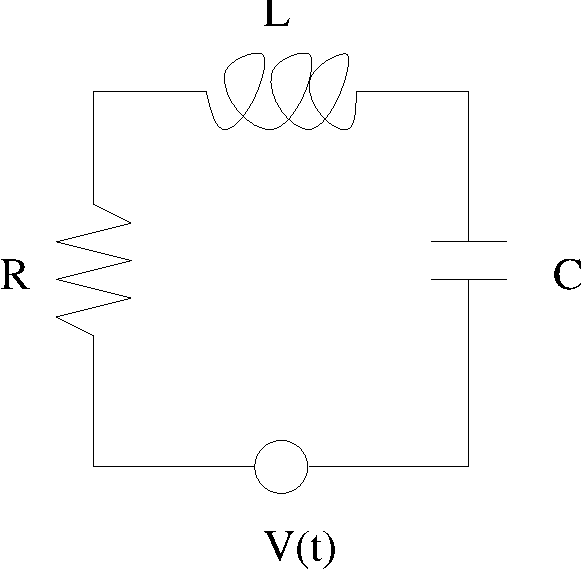
\includegraphics[width=2.0in]{../figures/rcl.pdf}}
           \caption{An RLC circuit with resistance $R$, inductance $L$,
	   capacitance $C$, and a voltage source $V(t)$.}
           \label{fig:rcl}
\end{figure}

We describe the behavior of the circuit by the voltage drop $x(t)$ at the 
capacitor.  Kirchhoff's Laws\index{Kirchhoff's laws} 
for electric circuits show that $x(t)$ satisfies 
the second order differential equation
\begin{equation}  \label{e:eleccirc}
\frac{1}{CL}V(t) = \frac{d^2x}{dt^2}(t) + \frac{R}{L}\frac{dx}{dt}(t) + 
\frac{1}{CL}x(t),
\end{equation}
as we now explain.   {\em Kirchhoff's Voltage 
Law\/}\index{Kirchhoff's laws} states that at each
instant of time the voltage $V(t)$ produced at the source is
equal to the sum of the voltage drops at the three elements of
the circuit.  So, if we denote the voltage drops at the coil\index{coil}
by $V_{coil}$ and at the resistor\index{resistor} by $V_{resistor}$, then 
we have 
\begin{equation}  \label{e:kirchhoff}
V(t) = V_{coil}(t) + V_{resistor}(t) + x(t),
\end{equation}
recalling that $x(t)$ is the voltage drop at the capacitor\index{capacitor}.

Let $I(t)$ be the current through the system.  Then 
\begin{itemize}
\item[(a)]  The voltage drop in a capacitor is proportional to the charge 
difference $Q_{capacitor}$ between the two plates:
\[
x(t) = \frac{1}{C}Q_{capacitor},
\]
where $C$ is the {\em capacitance\/} measured in farads.  The charge 
difference itself is related to the current by 
\[
I = \frac{dQ_{capacitor}}{dt} = C\frac{dx}{dt}.
\]
\item[(b)]  The voltage drop at a resistor is proportional to the current:	
\[
V_{resistor} = RI = RC\frac{dx}{dt},
\]
where $R$ is the {\em resistance\/} measured in ohms.
\item[(c)]  The voltage drop in a coil\index{coil} is given by 
{\em Faraday's Law}\index{Faraday's law}; 
the drop is proportional to the rate of change of the current\index{current}:
\[
V_{coil} = L\frac{dI}{dt} = LC\frac{d^2x}{dt^2},
\]
where $L$ is the inductance of the coil measured in henrys.
\end{itemize}

Combining (a,b,c) with \eqref{e:kirchhoff}, we obtain the differential equation:
\[
V(t) = LC\ddot{x} + RC\dot{x} +  x.
\]
After dividing by $LC$, we obtain the second order equation \eqref{e:eleccirc};
and, on setting 
\[
a = \frac{R}{L}, \quad b = \frac{1}{CL}, \AND g(t) = \frac{1}{CL}V(t),
\] 
we have an initial value problem in the form \eqref{e:2ndforced}.

A typical input at the voltage source\index{voltage source} 
(associated to alternating current) is 
a $2T$-periodic square wave with amplitude $A>0$ defined by periodicity and
\[
V(t) = \left\{\begin{array}{rl} A & 0<t\leq T\\
			       -A & T<t\leq 2T.
	\end{array}\right.
\]
See Figure~\ref{fig:sq}.  We will see how to use Laplace transforms to solve 
second order equations with a discontinuous forcing\index{forcing!discontinuous} 
of this type.  Indeed,
it is the possibility of using Laplace transforms to solve linear equations 
with piecewise smooth forcing terms\index{forcing!piecewise smooth} that is 
the main strength of Laplace
transforms.

\begin{figure}[htb]
           \centerline{%
           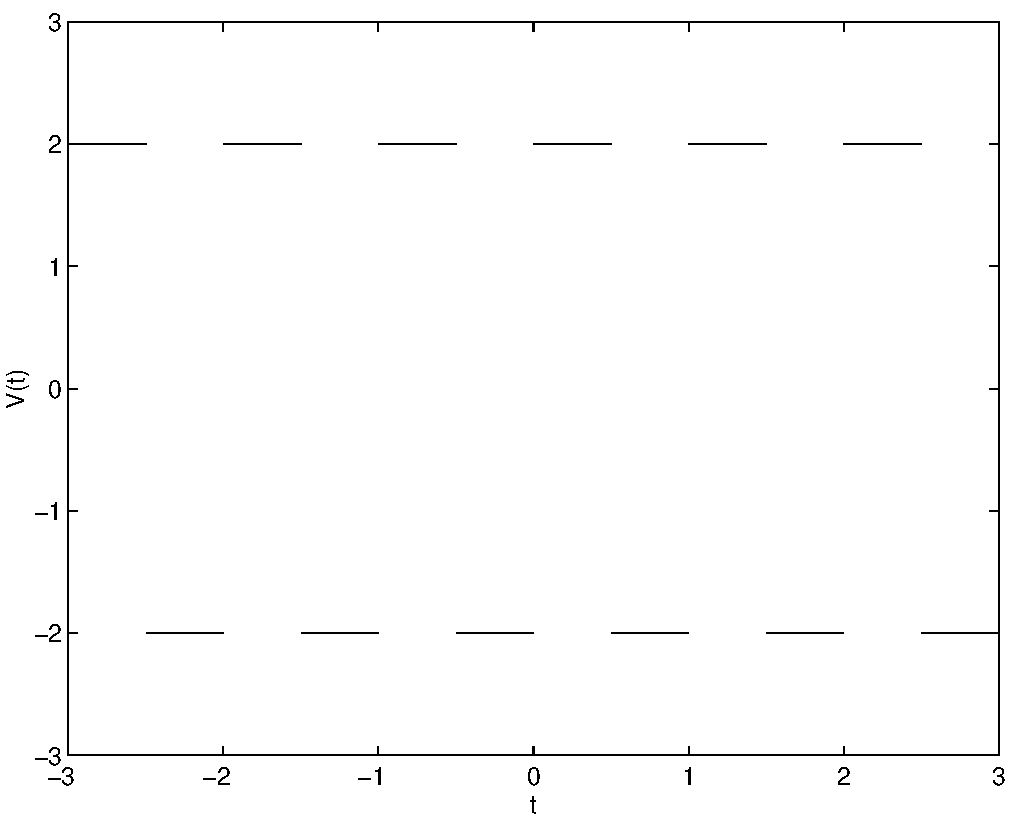
\includegraphics[width=3.0in]{../figures/sq.pdf}}
           \caption{A 1-periodic square wave $V(t)$ of amplitude $A=2$.}
           \label{fig:sq}
\end{figure}


\subsection*{Piecewise Smooth Periodic Forcing}
\index{forcing!piecewise smooth!periodic}

We now show how Laplace transforms can be used to solve second order
equations with periodic discontinuous forcing.  As an example we consider
the equation \eqref{eq:ivH1} where the external force $g(t)$ is
given by
\begin{equation}
g(t) =  
\left\{\begin{array}{cl} 1 & \mbox{for $t \in [2k,2k+1]$} \\ 
		0 & \mbox{for $t \in [2k+1,2k+2]$} \end{array} \right.
(k=0,1,2,\ldots).
\end{equation}
We begin by computing the Laplace transform of $g(t)$. Using the 
definition we obtain
\begin{eqnarray*}
{\cal L}[g] & = & \int_0^\infty e^{-st} g(t)\, dt\\
&=& \sum_{k=0}^\infty \int_k^{k+1} e^{-st} g(t)\, dt\\
&=& \sum_{k=0}^\infty \int_{2k}^{2k+1} e^{-st}\, dt,
\end{eqnarray*}
since $g(t)$ vanishes for $t \in [2k+1,2k+2]$. Performing the
integrations leads to
\begin{eqnarray*}
{\cal L}[g] & = & \frac{1}{s}\sum_{k=0}^\infty \left(e^{-2sk}-e^{-s(2k+1)}\right)\\
&=& \frac{1}{s}\sum_{k=0}^\infty (1-e^{-s})e^{-2sk}\\
&=& \frac{1}{s} (1-e^{-s}) \frac{1}{1-e^{-2s}}\\
&=& \frac{1}{s(1+e^{-s})}.
\end{eqnarray*}
Hence an application of the Laplace transform to the differential equation 
\eqref{eq:ivH1} gives
\[
s^2{\cal L}[x]-s + 4{\cal L}[x] = {\cal L}[g] = \frac{1}{s(1+e^{-s})},
\]
and solving this for ${\cal L}[x]$ leads to
\[
{\cal L}[x] = \frac{1}{s(s^2 +4)(1+e^{-s})} + \frac{s}{s^2 +4}.
\]
It remains to compute the inverse Laplace transform\index{Laplace transform!inverse} 
of the first term.  For this
we observe that for real numbers $x$ with $|x|<1$ the following identity holds:
\[
\frac{1}{1+x} = 1-x+x^2-x^3+x^4-\cdots = \sum_{k=0}^\infty (-1)^k x^k.
\]
Hence, for positive $s$,
\[
\frac{1}{1+e^{-s}} = \sum_{k=0}^\infty (-1)^k e^{-sk},
\]
and it follows that
\begin{eqnarray*}
{\cal L}[x] &=&\frac{1}{s(s^2 +4)}\sum_{k=0}^\infty (-1)^k e^{-sk} + \frac{s}{s^2 +4}\\
&=& \frac{1}{4}\left(\frac{1}{s}-\frac{s}{s^2+4}\right)
    \sum_{k=0}^\infty (-1)^k e^{-sk} + \frac{s}{s^2 +4}\\
&=& \frac{1}{4}\left(\frac{1}{s}+\frac{3s}{s^2+4}+
   \left(\frac{1}{s}-\frac{s}{s^2+4}\right) \sum_{k=1}^\infty (-1)^k e^{-sk}\right)\\
&=& \frac{1}{4}\left(\frac{1}{s}+\frac{3s}{s^2+4}+
   \sum_{k=1}^\infty (-1)^k \frac{e^{-sk}}{s}-
   \sum_{k=1}^\infty (-1)^k \frac{e^{-sk}s}{s^2+4}\right).
\end{eqnarray*} 
Now we have derived an expression for ${\cal L}[x]$ in which we can compute the
inverse Laplace transform for each of the individual summands.  Using 
Table~\ref{tab:Laplist} and Proposition~\ref{prop:eHcLap2} we obtain
\begin{eqnarray*}
x(t)&=&\frac{1}{4}\left(1+3\cos(2t)+\sum_{k=1}^\infty (-1)^k H_k(t)
       -\sum_{k=1}^\infty (-1)^k H_k(t)\cos(2(t-k))\right)\\
&=&\frac{1}{4}\left(1+3\cos(2t)+\sum_{k=1}^\infty (-1)^k H_k(t)(1-\cos(2(t-k)))\right)\\
&=&\frac{1}{4}\left(1+3\cos(2t)+2\sum_{k=1}^\infty (-1)^k H_k(t)\sin^2(t-k))\right).
\end{eqnarray*}
In Figure~\ref{fig:lapperi} we show the solution for $t\in [0,20]$.  Observe 
that this solution is certainly not periodic in time.  Indeed, since the 
internal frequency\index{frequency!internal} of equation \eqref{eq:ivH1} is 
$1/\pi$ and the frequency of the external periodic forcing is $1/2$ we expect 
to obtain a quasiperiodic motion\index{motion!quasiperiodic}.
\begin{figure}[htb]
           \centerline{%
           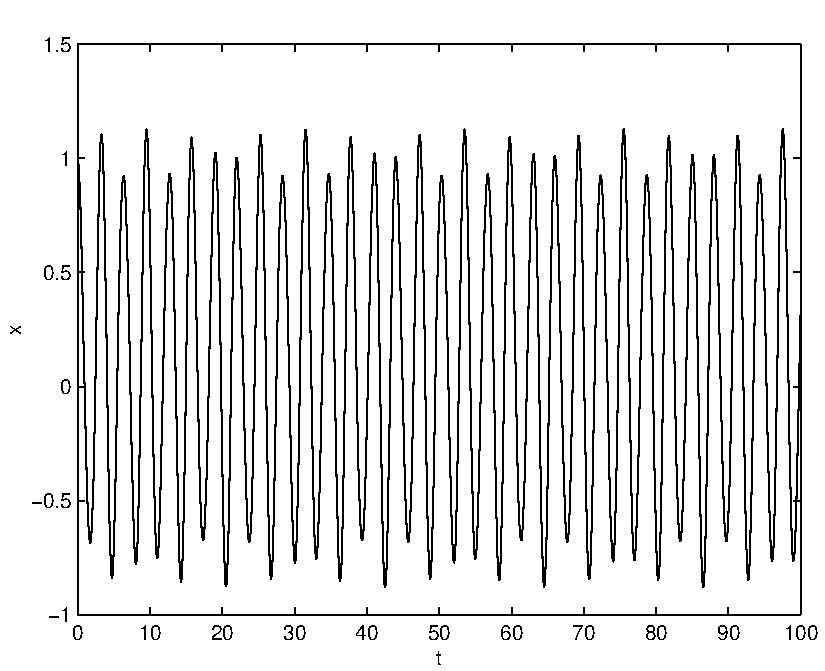
\includegraphics[width=3.5in]{../figures/lapperi.pdf}}
           \caption{The solution of the initial value problem
	   \protect\eqref{eq:ivH1} where the external force is
   	   given by a periodic discontinuous function.}
           \label{fig:lapperi}
\end{figure}






\end{document}
